\documentclass[14pt,a4paper]{extarticle}
\usepackage[T1]{fontenc}
\usepackage[utf8]{inputenc}
\usepackage[scaled]{helvet}
\renewcommand{\familydefault}{\sfdefault}
\usepackage{amsmath}
\usepackage{sansmath}
\sansmath
\usepackage[a4paper,margin=2cm]{geometry}
\usepackage{tikz}
\usetikzlibrary{angles,quotes,patterns}
\usepackage{array}
\pagestyle{empty}
% Zweite Seite: 5-mm-Kästchen, 1 cm Rand
\newcommand{\kaestchen}{\newpage\null\begin{tikzpicture}[remember picture,overlay]
\begin{scope}[shift={(current page.south west)}]\draw[step=5mm, black!45, line width=0.3pt] (1cm,1cm) grid (20cm,28.5cm);\draw[black!45, line width=0.3pt] (1cm,1cm) rectangle (20cm,28.5cm);\end{scope}
\end{tikzpicture}}
\setlength{\parindent}{0pt}
\hyphenpenalty=10000

% Nur Schwarz und Grau, die Blätter werden schwarz-weiß kopiert.
% Merkblock: Begriff und Text links, Zeichnung rechts.
\newcommand{\bl}{0.5}
\newcommand{\block}[3]{%
\begin{minipage}[c]{\bl\textwidth}\raggedright{\Large\bfseries #1\par}\medskip #2\end{minipage}\hfill
\begin{minipage}[c]{\dimexpr0.97\textwidth-\bl\textwidth\relax}\centering #3\end{minipage}\par}

\renewcommand{\bl}{0.47}
\begin{document}

{\LARGE\bfseries Winkelsumme im Dreieck und Viereck\par}
\vspace{0.9cm}

\block{Dreieck}{%
Die drei Innenwinkel eines Dreiecks sind zusammen $180^\circ$ groß.
\[
\begin{array}{r@{\;=\;}l@{\quad}l}
\alpha + \beta + \gamma & 180^\circ & \mid -\alpha - \beta\\[2pt]
\gamma & \rlap{$180^\circ - \alpha - \beta$} &
\end{array}
\]
Beispiel: $\alpha = 50^\circ$, $\beta = 60^\circ$\par\smallskip
$\gamma = 180^\circ - 50^\circ - 60^\circ = 70^\circ$}{%
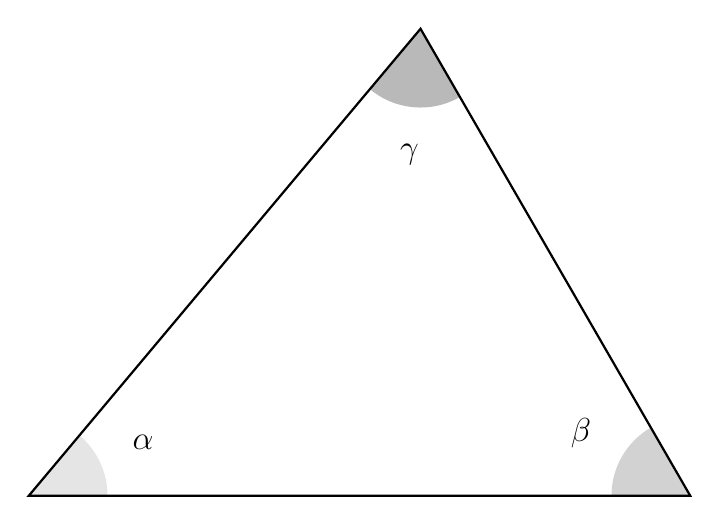
\begin{tikzpicture}[scale=2.1]
  \coordinate (A) at (0,0); \coordinate (B) at (4,0); \coordinate (C) at (2.369,2.824);
  \pic[fill=gray!20, angle radius=1.0cm, "\large$\alpha$", angle eccentricity=1.6] {angle=B--A--C};
  \pic[fill=gray!35, angle radius=1.0cm, "\large$\beta$", angle eccentricity=1.6] {angle=C--B--A};
  \pic[fill=gray!55, angle radius=1.0cm, "\large$\gamma$", angle eccentricity=1.6] {angle=A--C--B};
  \draw[thick] (A) -- (B) -- (C) -- cycle;
\end{tikzpicture}}

\vspace{1cm}

\block{Viereck}{%
Die vier Innenwinkel eines Vierecks sind zusammen $360^\circ$ groß. Eine Diagonale teilt das Viereck in zwei Dreiecke: $2 \cdot 180^\circ = 360^\circ$.
\[
\begin{array}{r@{\;=\;}l@{\quad}l}
\alpha + \beta + \gamma + \delta & 360^\circ & \mid -\alpha - \beta - \gamma\\[2pt]
\delta & \rlap{$360^\circ - \alpha - \beta - \gamma$} &
\end{array}
\]
Beispiel: $\alpha = 80^\circ$, $\beta = 100^\circ$, $\gamma = 70^\circ$\par\smallskip
$\delta = 360^\circ - 80^\circ - 100^\circ - 70^\circ = 110^\circ$}{%
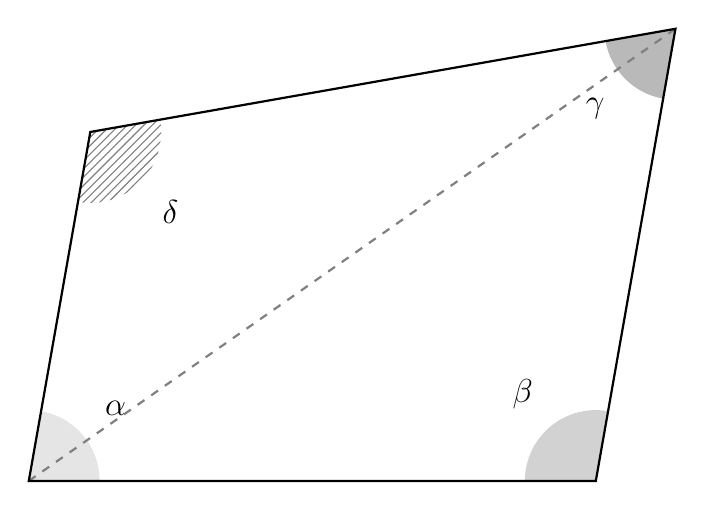
\begin{tikzpicture}[scale=1.8]
  \coordinate (A) at (0,0); \coordinate (B) at (4,0); \coordinate (C) at (4.562,3.190); \coordinate (D) at (0.434,2.462);
  \pic[fill=gray!20, angle radius=0.9cm, "\large$\alpha$", angle eccentricity=1.6] {angle=B--A--D};
  \pic[fill=gray!35, angle radius=0.9cm, "\large$\beta$", angle eccentricity=1.6] {angle=C--B--A};
  \pic[fill=gray!55, angle radius=0.9cm, "\large$\gamma$", angle eccentricity=1.6] {angle=D--C--B};
  \pic[pattern=north east lines, pattern color=gray, angle radius=0.9cm, "\large$\delta$", angle eccentricity=1.6] {angle=A--D--C};
  \draw[thick, dashed, gray] (A) -- (C);
  \draw[thick] (A) -- (B) -- (C) -- (D) -- cycle;
\end{tikzpicture}}

\vspace{1cm}

{\Large\bfseries Aufgaben im Heft\par}
\medskip
Buch S.\,65 Nr.\,1, 2, 3\par\smallskip
Buch S.\,66 Nr.\,1, 2, 3, 4\par\smallskip
Buch S.\,67 Nr.\,1, 2, 3, 4, 5
\kaestchen
\end{document}
